\documentclass{report}

% !TEX root = ../main.tex

\usepackage[english]{babel}
\usepackage{varioref}
\usepackage{chemfig}
\usepackage{circuitikz}
\usepackage{tikz}
\usepackage{tikzscale}
\usepackage{environ}
\usepackage{float}
\usepackage{url}
\usepackage{adjustbox}
\usepackage{siunitx}
\usepackage{svg}
\usepackage{subcaption}
\usepackage{listings}
\usepackage[parfill]{parskip}
\usepackage[noabbrev,capitalize]{cleveref}
\usepackage[compact, nobottomtitles*]{titlesec}

\usetikzlibrary{shapes,arrows,calc}

\DeclareCaptionLabelFormat{bold}{\textbf{(#2)}}
\captionsetup{subrefformat=bold}

% For easier referring like \fref, \tref, \eref
\newcommand{\tref}[1]{\vref{#1}}
\newcommand{\fref}[1]{\vref{#1}}
\newcommand{\eref}[1]{\vref{#1}}
\newcommand{\lref}[1]{\vref{#1}}
\renewcommand{\lstlistingname}{Code}
\crefname{listing}{Code}{Code}

\lstset{
   breaklines=true,
   frame=single,
   basicstyle=\small\ttfamily,
   captionpos=b
 }

 \makeatletter
\def\@makechapterhead#1{%
  \vspace*{50\p@}%
  {\parindent \z@ \raggedright \normalfont
    \ifnum \c@secnumdepth >\m@ne
      \if@mainmatter
        %\huge\bfseries \@chapapp\space \thechapter
        \Huge\bfseries \thechapter.\space%
        %\par\nobreak
        %\vskip 20\p@
      \fi
    \fi
    \interlinepenalty\@M
    \Huge \bfseries #1\par\nobreak
    \vskip 40\p@
  }}
\makeatother

 \widowpenalties 1 10000


\title{Strand displacement neural networks and RNA translators}
\author{Daniel Svane Nielsen}
\date{\today}
\begin{document}

  \maketitle

  \begin{abstract}
  The purpose of this project is to investigate a previously designed method of creating strand displacement neural networks, and combine them with RNA translation, for possible future use in general biosensors and molecular computers. The strand displacement neural network is created using a DNA motif called the seesaw gate. The seesaw gate requires some specific domains to function, so to use arbitrary sequences as input to the network, the sequences have to be translated. This report first goes through the theory of neural networks and strand displacement reactions, and later applies it for recreating the seesaw neural network. It is successfully shown that simple neural networks (perceptrons) can be trained to realize specific logic operations based on their truth tables, but with some limitations. The RNA translator was intended to be transcribed from a DNA template, and the displacement reactions tested using a fluorescent reporter. It was not possible to transcribe the RNA strands, so no succesful RNA translation is shown in this report.
  \end{abstract}


  \tableofcontents

  \chapter{Introduction}
  % !TEX root = ../main.tex
Logic circuits using DNA and RNA has many interesting applications in diagnostics and treatment. An example is cancer detection, where miRNA's can be used as biomarkers \cite{Peng2016}. These biomarkers can be used as inputs for logic circuits, which can be designed to activate fluorescence signals \cite{Seelig2006} or enzymes \cite{Engelen2016} when combinations of biomarkers are present or absent. For example, a circuit could be designed to activate when 2 unique miRNA's are present at the same time, or when a certain protein is present.

A different approach to building logic circuits is using neural networks. One of the advantages of this approach, is that large-scale networks does not have to be designed by someone with knowledge of logic gates and circuitry. The inputs of the circuit simply have to be defined along with the required output, and the neural network can be trained to give the desired functionality.

The neural network approach to strand displacement circuits has already been developed \cite{Qian2011}. The design is based on the seesaw gate motif, which requires that the inputs to the network must be have very specific sequences. To use custom input sequences, like the miRNAs from cancer cells, the sequences have to be translated. This has also already been done, using two linked strand displacement reactions \cite{Picuri2009}.

This project is split into two parts.

The first part aims to lay out the groundwork for a software where the miRNAs one wishes to detect can be entered. The strands and concentrations required for a neural network that implements a desired truth table is then calculated, and could be readily ordered and used as a biosensor.

The second part aims to translate one RNA sequence into another RNA sequence, and measuring the outcome by a fluorescent reporter. This is almost identical to the experiment in \cite{Picuri2009}, but using RNA instead of DNA in the translation reactions. This is mostly done to show that the translators could also use RNA, but also to get some experience in a laboratory.

  %
  %% !TEX root = ../main.tex
\section{Logic gates}
Logic gates in electric circuits are usually made using transistors. They can take boolean inputs (0 or 1) and output another boolean signal depending on the inputs and type of logic gate. An example of an AND logic gate can be seen in figure \ref{and_gate}.

\begin{figure}[H]
\centering
\begin{tabular}{cccc}
    \begin{circuitikz}[baseline=-0.7ex]
        \draw (0,0) node[and port] (and1) {}
        (and1.in 1) [anchor=east] node {A}
        (and1.in 2) [anchor=east] node {B}
        (and1.out) [anchor=west] node {O};
    \end{circuitikz}
    &
    $\begin{array}{ccc}
        A & B & O \\ \hline
        0 & 0 & 0 \\
        0 & 1 & 0 \\
        1 & 0 & 0 \\
        1 & 1 & 1 \\
    \end{array}$
\end{tabular}

\label{and_gate}
\caption{To the left, an AND gate with inputs A and B, and output O. To the right, the truth table for the AND gate.}
\end{figure}

Different gates exist, with different truth tables. These gates can be combined into more complex circuits, like calculators and integrated circuits, which exist in all modern computers.



  \chapter{Theory}
  % !TEX root = ../main.tex
\section{Strand displacement}

Strand displacement can be used to implement DNA devices which can be used in molecular computing \cite{Zhang2011}. It uses the predictability of Watson-Crick base pairing (A pairs with T, C pairs with G) of the nucleotides of DNA to design reactions. When the nucleotides of two strands of DNA base pair with each other, the complex will have a certain free energy. By introducing another strand which will pair stronger in the complex (give a lower free energy), the original strand can be displaced, as seen in \fref{strand_displacement}.

\begin{figure}[H]
\centering
\includegraphics[width=\textwidth]{figures/strand_displacement.tikz}
\caption{Strand displacement reaction where strand 1 base pairs at a lower free energy with strand 2, and displaces strand 3. The arrow denotes the strands 3' end.}
\label{strand_displacement}
\end{figure}

The reaction in \fref{strand_displacement} can be simplified by leaving out the specific bases, and instead naming each base pairing region. The same reaction as in \fref{strand_displacement} can be seen in its simplified version in \fref{strand_displacement_simple}.

\begin{figure}[H]
\centering
\includegraphics[width=\textwidth]{figures/strand_displacement_simple.tikz}
\caption{Simplified view of the reaction from \fref{strand_displacement}. The sequence of nucleotides is replaced with a domain name. The asterix on the sequence name denotes that it is the reverse complement of the normal sequence (a$^*$ is the reverse complement of a).}
\label{strand_displacement_simple}
\end{figure}

The result of the reaction in \fref{strand_displacement_simple}, is that the strand $bc$ is only single-stranded when displaced by the strand $ab$. The reaction can then be seen as a YES gate with input $ab$ and outout $bc$. Why this is useful in molecular computing is not immediately apparent, but the strand displacement technique can be extended to larger reactions. A more interesting application is the AND gate seen in \fref{strand_displacement_and}.

\begin{figure}[H]
\centering
\includegraphics[width=\textwidth]{figures/and_gate_dna.tikz}
\caption{An AND gate made with strand displacement. After two strand displacements by the input strands $a^*b^*c^*$ and $bcdf$, the ouput strand $def$ is released and can react in further strand displacement reactions with other logic gates, or activate enzymes and fluorescence signals. Without either of the input strands, the output will not be displaced. Adapted from \cite{Zhang2011}.}
\label{strand_displacement_and}
\end{figure}

The actual concentrations of each of the strand species when reacting, can be predicted by the free energy of each complex \cite{Zhang}, but the time it takes for the reaction to take place is harder to predict. It has been shown that the reaction speed is exponentially dependent on the toehold length for short toeholds \cite{Zhang}. A toehold, for example, is the single stranded region of the strand 2 + strand 3 complex in \fref{strand_displacement}. To do time analysis of larger strand displacement networks, software like Visual DSD \cite{Lakin2011} can be used.

  % !TEX root = ../main.tex
\section{Neural networks}
\subsection{In silico neural networks}
Artificial neural networks (referred to just as neural networks) is a software implementation of the connection of neurons in the brain. In computer science they can be used to solve a wide variety of problems, like character and facial recognition. They present an advantage over conventional programmatic methods, as they don't need explicit coding for each new problem. There exist many different implementations of neural networks, but in the case of the perceptron (also known as feed-forward neural network), it only needs to know the inputs and the matching outputs to train itself. An example usage showing character recognition can be seen in figure \ref{neuralnetwork_example}.

\begin{figure}[H]
\centering
\includegraphics[width=\columnwidth]{images/neuralnetwork_example.png}
\caption{An example usage of a neural network recognizing the handdrawn letter "a". The typical approach is to segment the area into a grid. Only 2x2 is shown here for simplification, but usually larger grids are used. The average color of each segment is calculated, and fed into a neural network, which has been trained to output "a", when presented an input resembling the handdrawn version.}
\label{neuralnetwork_example}
\end{figure}

The neural network works by simulating the functionality of the brain, by connecting neurons together by varying strength. Continuing the example from figure \ref{neuralnetwork_example}, the 4 segments are fed into 4 input neurons (see figure \ref{neuralnetwork_neurons}). The 4 input neurons are connected to an output neuron by varying strength, much like the synapses of the natural neuron. If the weighted inputs sum exceed the threshold of the output neuron, it will activate. In this simplified example, the output neurons activation is of limited value, as it can only give a yes or no answer to if the input resembles an "a".

\begin{figure}[H]
\centering
\includegraphics[width=200]{images/neuralnetwork_neurons.png}
\caption{}
\label{neuralnetwork_neurons}
\end{figure}

 In a more practical example, the network would have enough input neurons to accommodate a 100x100 grid (10,000 input neurons), have some layers of neurons between the input and output (hidden layers), and enough output neurons to represent binary encoded characters (see figure \ref{neuralnetwork_ocr}).

 \begin{figure}[H]
 \centering
 \includegraphics[width=\columnwidth]{images/neuralnetwork_ocr.png}
 \caption{}
 \label{neuralnetwork_ocr}
 \end{figure}

\subsection{In vitro neural networks}
It has previously been shown that the function of the artificial neuron can also be implemented using strand displacement reactions. The system is based on the seesaw gate motif \cite{Qian}, and can fullfill most of the functionality of a real neuron \cite{Qian2011}.

%INSERT GENERAL INFORMATION ABOUT THE SEESAW WITH TOEHOLDS HERE

\subsubsection{Seesaw gate}

The seesaw gate is a catalytic gate with a threshold, designed for use in scalable strand displacement circuits.


ALSO A SUMMARY OF INPUT WEIGHT, SUMMATION, THRESHOLDING

\subsubsection{Thresholding}
In the natural neuron, the neuron will activate when its inputs exceeds a threshold. This is implemented using a threshold gate which will bind the input and prevent it from reacting downstream in the network. If the threshold gate concentration is higher than the input concentration, the input will be suppressed by the threshold. If the threshold gate concentration is lower than the input concentration, not all of the input is suppressed, and will be able to react further downstream in the network.

% \begin{subfigure}{.49\columnwidth}
%   \centering
%   \includegraphics[width=\linewidth]{images/transcription_annealed_nostain.png}
%   \caption{Not stained}
% \end{subfigure}

\begin{figure}[H]
  \begin{subfigure}[t]{.49\columnwidth}
    \centering
\adjustbox{width=\linewidth} {
% !TEX root = ../main.tex

\begin{tikzpicture}[baseline=-110pt]

\def\inputstrand(#1,#2){
  \begin{scope}[shift={(#1,#2)}]
    \draw[-|](0, 0) -- node[above] {$S_1$} (2, 0);
    \draw[-|](2, 0) -- node[above] {$T$} (3, 0);
    \draw[->](3, 0) -- node[above] {$S_2$} (5, 0);
  \end{scope}
}

% \node at (6, 0) {$+$};

\def\thresholdbot(#1,#2){
  \begin{scope}[shift={(#1,#2)}]
    \draw[<-](7, -0.1) -- node[below] {$s_1^*$} (8, -0.1);
    \draw[|-](8, -0.1) -- node[below] {$T^*$} (9, -0.1);
    \draw[|-](9, -0.1) -- node[below] {$S_2^*$} (11, -0.1);
  \end{scope}
}

\def\thresholdtop(#1,#2){
  \begin{scope}[shift={(#1,#2)}]
    \draw[->](9, 0.1) -- node[above] {$S_2$} (11, 0.1);
  \end{scope}
}

\inputstrand(0,0)
\thresholdbot(0,0)
\thresholdtop(0,0)

\draw[->](6, -2) -- (6, -4);

\inputstrand(0,-5)
\thresholdbot(-6,-5.1)
% \node at (6, -5.1) {$+$};
\thresholdtop(-1,-5.2)

\node[align=center] at (2.5, -1.5) {Input strand};

\node[align=center] at (9, -1.5) {Threshold gate};

\node[align=center] at (9, -6) {Waste};

% \def\strandtwo(#1,#2){
%   \begin{scope}[shift={(#1,#2)}]
%     \draw[<-](4,0.3) -- node[above] {d} (5.9,0.3);
%     \node[label=above:{e}] at (6,1) {};
%     \draw plot [smooth, tension=1] coordinates {(5.9, 0.3) (5.9, 0.4) (5.7, 0.7) (6, 1) (6.3, 0.7) (6.1, 0.4) (6.1, 0.3)};
%     \draw(6.1,0.3) -- node[above] {f} (8,0.3);
%   \end{scope}
% }

\end{tikzpicture}

}
\caption{Reaction of an input strand with a threshold gate. The product has no free toehold domain, and can't undergo reverse reaction. The waste has no toehold, and can't parcitipate in further reactions.}
\label{}
\end{subfigure}
\hfill
\begin{subfigure}[t]{.49\columnwidth}
  \centering
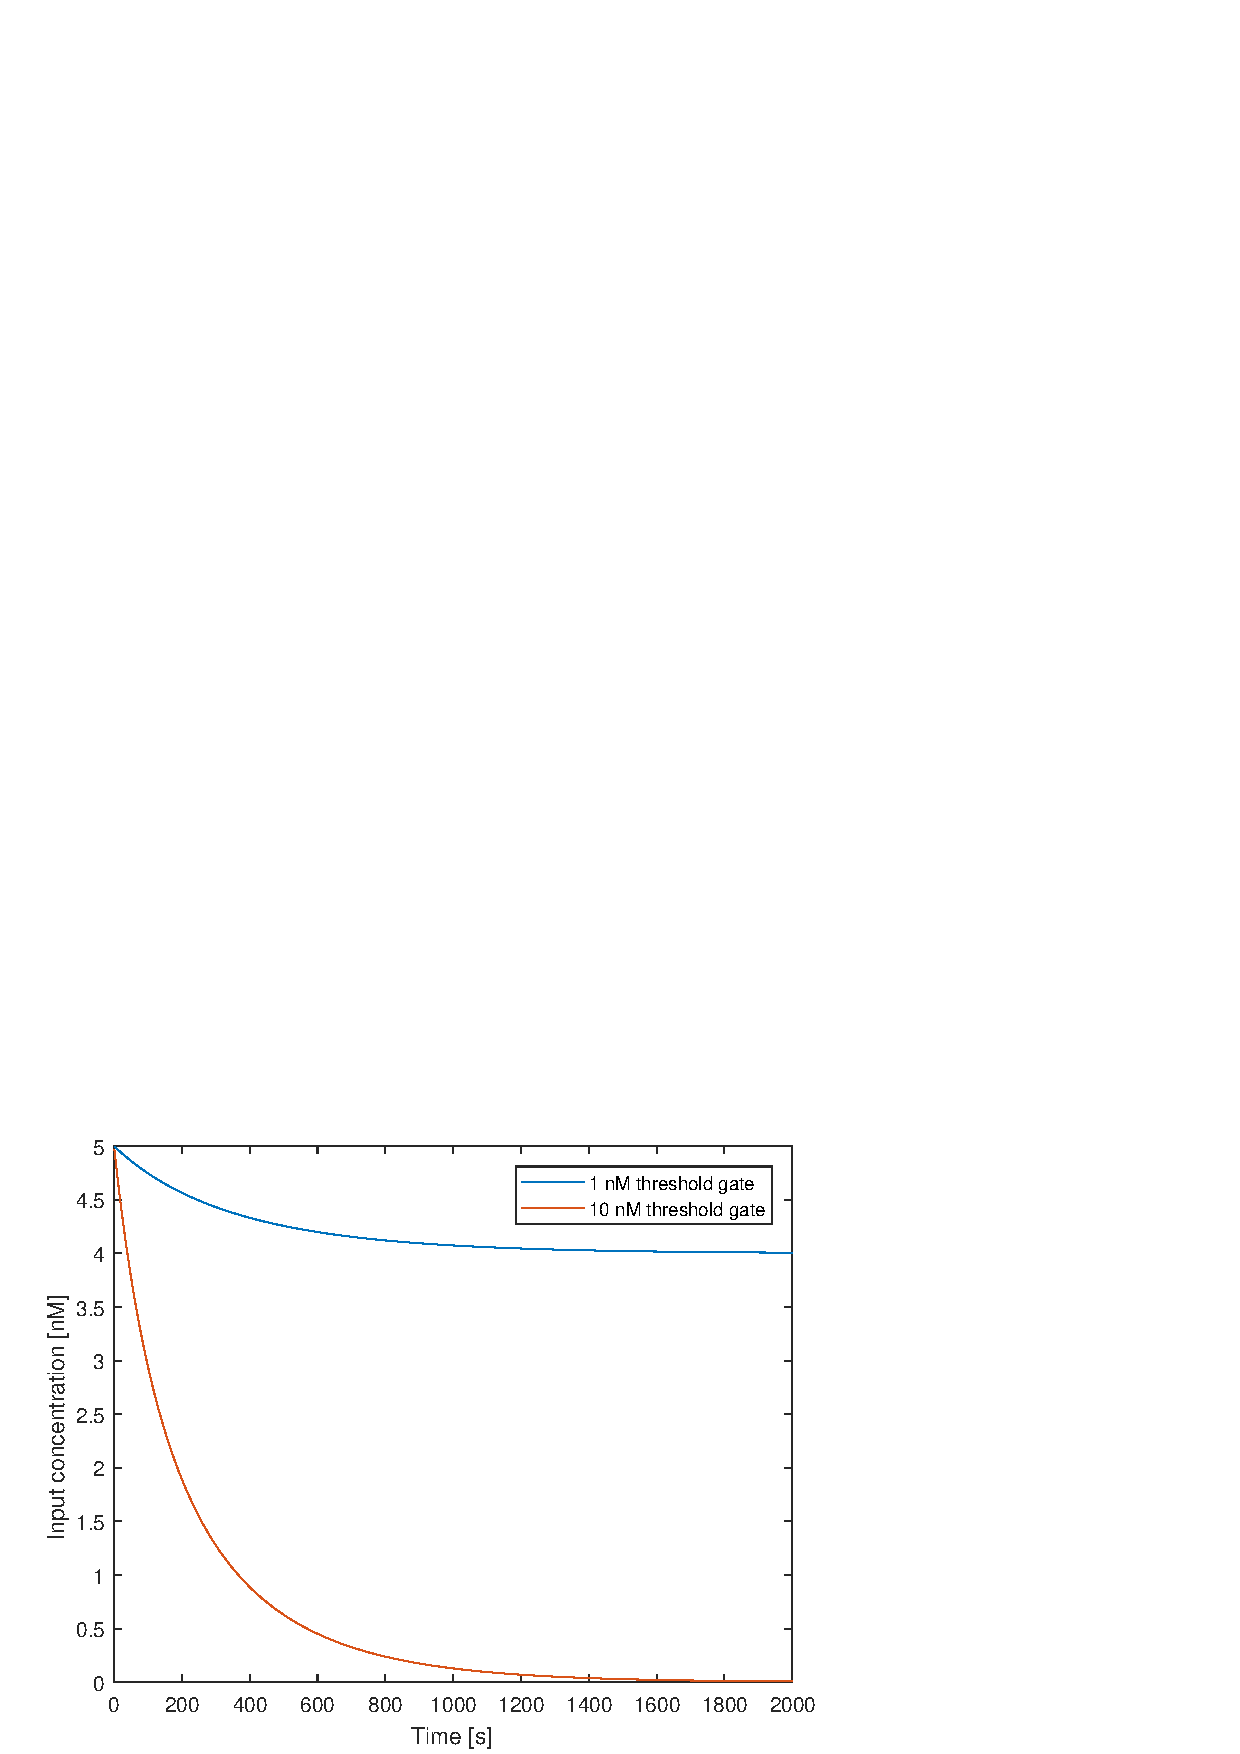
\includegraphics[width=\linewidth]{images/thresholding.png}
\caption{Time analysis of the concentration of input strand (5 nM start concentration). A threshold concentration higher than the input (red) will bind all input strand. A lower concentration (blue), will allow the input strand to participate in further displacement reactions.}
\label{}
\end{subfigure}
\end{figure}

\subsubsection{Integration}
The input to the neuron have to be collected before thresholding, as they don't have the same left recognition sequence. This is done through an integrating gate, which will collect all inputs with the same right recognition sequence, and release a common signal which can be thresholded.

\begin{figure}[H]
  \begin{subfigure}[t]{.49\columnwidth}
    \centering
\adjustbox{width=\linewidth} {
% !TEX root = ../main.tex

\begin{tikzpicture}[baseline=-80pt]

\draw[-|](0, 0) -- node[above] {$S_1$} (2, 0);
\draw[-|](2, 0) -- node[above] {$T$} (3, 0);
\draw[->](3, 0) -- node[above] {$S_2$} (5, 0);

\draw[-|](0, -3) -- node[above] {$S_3$} (2, -3);
\draw[-|](2, -3) -- node[above] {$T$} (3, -3);
\draw[->](3, -3) -- node[above] {$S_2$} (5, -3);

\node at (6, -1.7) {$+$};

\draw[-|](8, -1.5) -- node[above] {$S_2$} (10, -1.5);
\draw[-|](10, -1.5) -- node[above] {$T$} (11, -1.5);
\draw[->](11, -1.5) -- node[above] {$S_4$} (13, -1.5);

\draw[<-](7, -1.7) -- node[below] {$T^*$} (8, -1.7);
\draw[-|](8, -1.7) -- node[below] {$S_2^*$} (10, -1.7);
\draw[-|](10, -1.7) -- node[below] {$T^*$} (11, -1.7);

\node[align=center] at (2.5, -1) {Input 1};

\node[align=center] at (2.5, -4) {Input 2};

\node[align=center] at (10, -3.3) {Integration gate};

\node[align=center] at (10.5, 0) {Output};

\end{tikzpicture}

}
\caption{Reaction of 2 input strands with an integration gate. The input strands have the same right recognition sequence $S_2$, and will both displace the top strand of the integration gate, releasing the output.}
\label{}
\end{subfigure}
\hfill
\begin{subfigure}[t]{.49\columnwidth}
  \centering
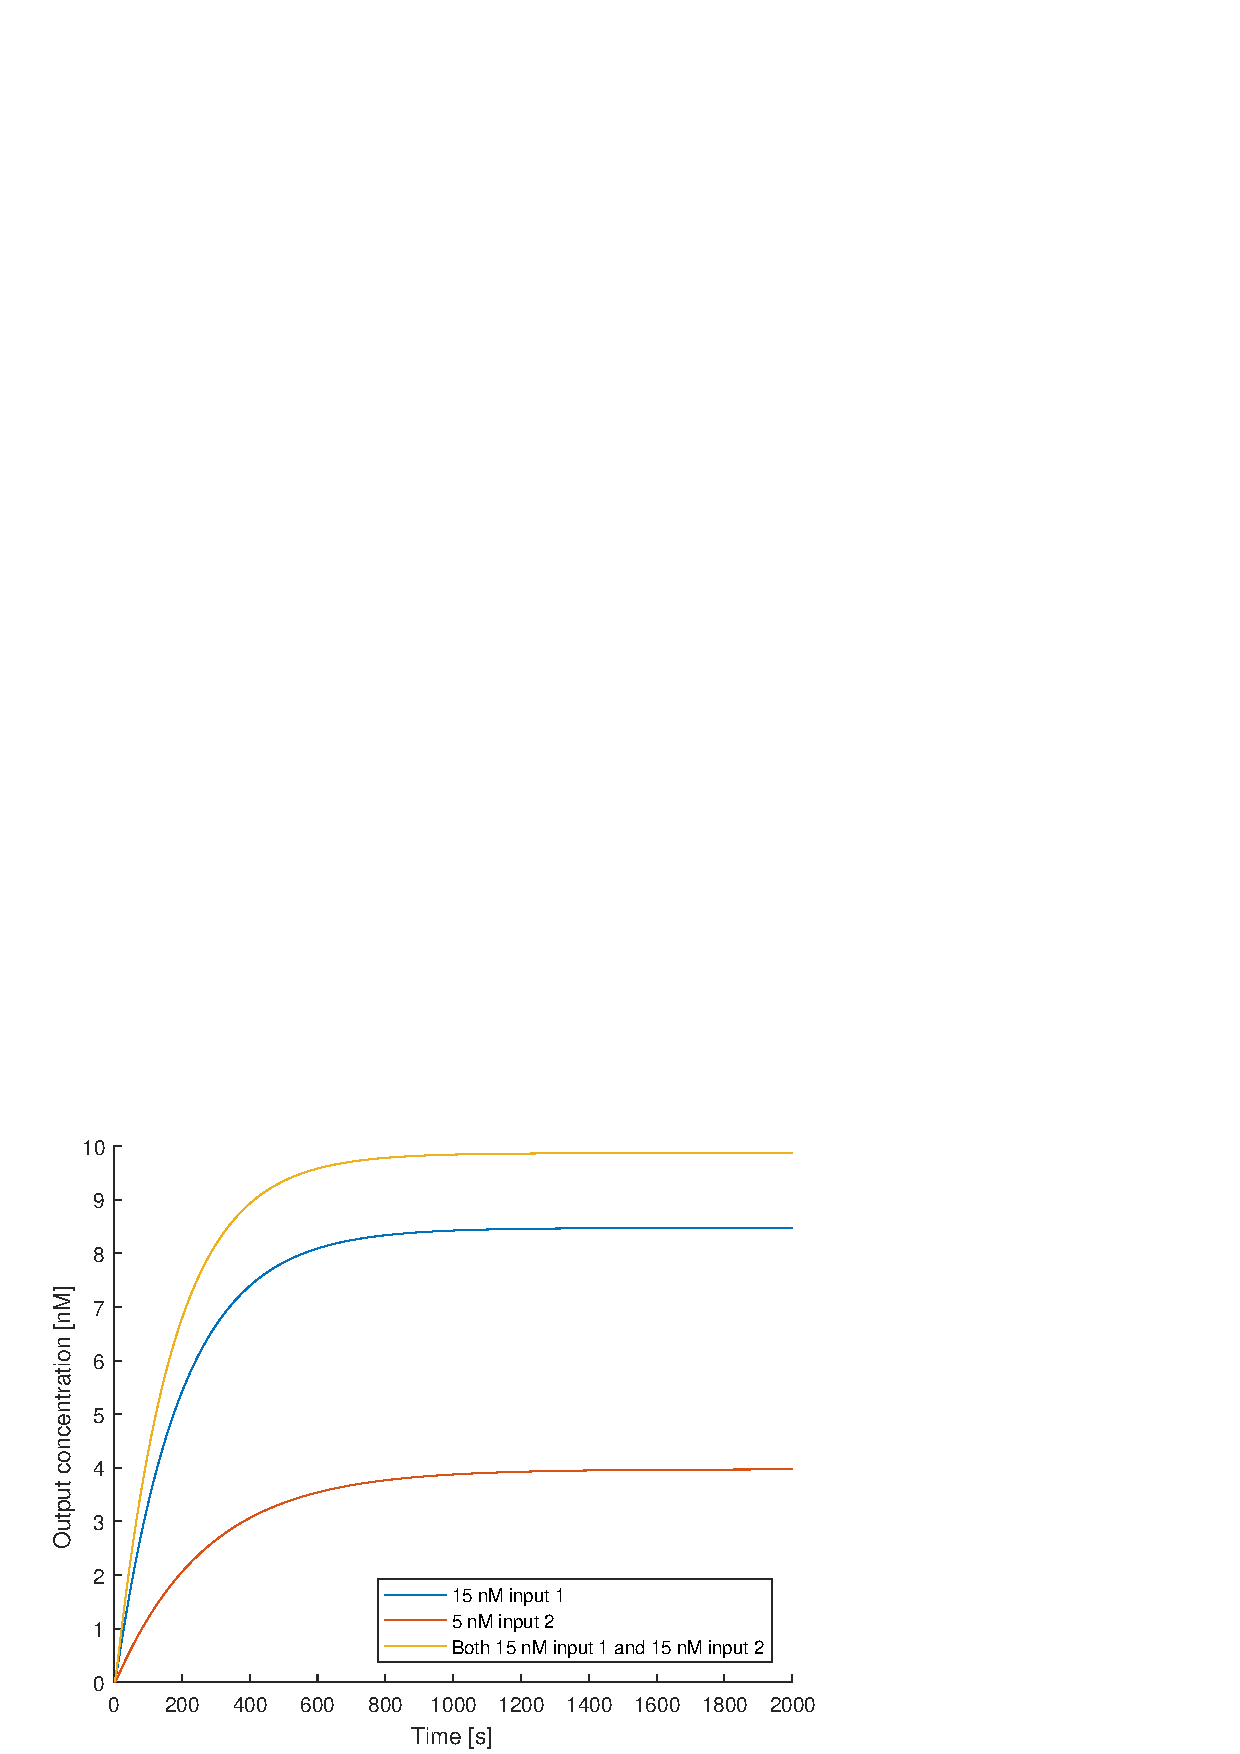
\includegraphics[width=\linewidth]{images/integration.png}
\caption{Time analysis of the concentration of the output strand. The concentration of the integration gate is 20 nM. The first input of 15 nM increases the output strand concentration, compared to the second input of 5 nM. When both strands are added the concentration of output increases further.}
\label{}
\end{subfigure}
\label{seesaw_integration}
\end{figure}

\subsubsection{Weighting}
The inputs to the gate are weighted using their concentration. By making the integration gates concentration the sum of all the input concentrations, a high concentration of one input strand will contribute more to the activation than that of a low concentration, as shown in \fref{seesaw_integration}.

The weight is decided by the concentration of output of a input neuron and its fuel strand. The fuel serves the purpose of pushing the output of one gate to its target concentration.

\begin{figure}[H]
  \begin{subfigure}[t]{.49\columnwidth}
    \centering
\adjustbox{width=\linewidth} {
% !TEX root = ../main.tex

\begin{tikzpicture}[baseline=-250pt]

\def\inputstrand(#1,#2){
  \begin{scope}[shift={(#1,#2)}]
    \draw[-|](0, 0) -- node[above] {$S_1$} (2, 0);
    \draw[-|](2, 0) -- node[above] {$T$} (3, 0);
    \draw[->](3, 0) -- node[above] {$S_2$} (5, 0);
  \end{scope}
}


\def\gatetop(#1,#2){

  \begin{scope}[shift={(#1,#2)}]
\draw[-|](1, -1.5) -- node[above] {$S_2$} (3, -1.5);
\draw[-|](3, -1.5) -- node[above] {$T$} (4, -1.5);
\draw[->](4, -1.5) -- node[above] {$S_3$} (6, -1.5);
\end{scope}
}

\def\gatebottom(#1,#2){

  \begin{scope}[shift={(#1,#2)}]
\draw[<-](0, -1.7) -- node[below] {$T^*$} (1, -1.7);
\draw[|-](1, -1.7) -- node[below] {$S_2^*$} (3, -1.7);
\draw[|-](3, -1.7) -- node[below] {$T^*$} (4, -1.7);
\end{scope}
}

\def\fuel(#1,#2){

  \begin{scope}[shift={(#1,#2)}]
\draw[-|](0, -3) -- node[above] {$S_2$} (2, -3);
\draw[-|](2, -3) -- node[above] {$T$} (3, -3);
\draw[->](3, -3) -- node[above] {$S_f$} (5, -3);
\end{scope}
}

\inputstrand(0,0)
\gatetop(-0.5,-1)
\gatebottom(-0.5,-1)
\fuel(0,-2)

\node[align=center] at (2.5, -0.5) {Input};
%
\node[align=center] at (2.5, -3.5) {Gate};

\node[align=center] at (2.5, -5.5) {Fuel};
\node[align=center] at (13, -3) {Output};
%
% \node[align=center] at (10, -2.7) {Integration gate};
%
% \node[align=center] at (10.5, -0.7) {Output};


\draw[->](7.5, -2.5) -- (8.5, -2.5);

\inputstrand(10,0)
\gatebottom(12,1.5)
\gatetop(9.5,-1)
\gatebottom(10,-3)
\fuel(11,-1.5)

\end{tikzpicture}

}
\caption{Reaction of 2 input strands with an integration gate. The input strands have the same right recognition sequence $S_2$, and will both displace the top strand of the integration gate, releasing the output.}
\label{}
\end{subfigure}
\hfill
\begin{subfigure}[t]{.49\columnwidth}
  \centering
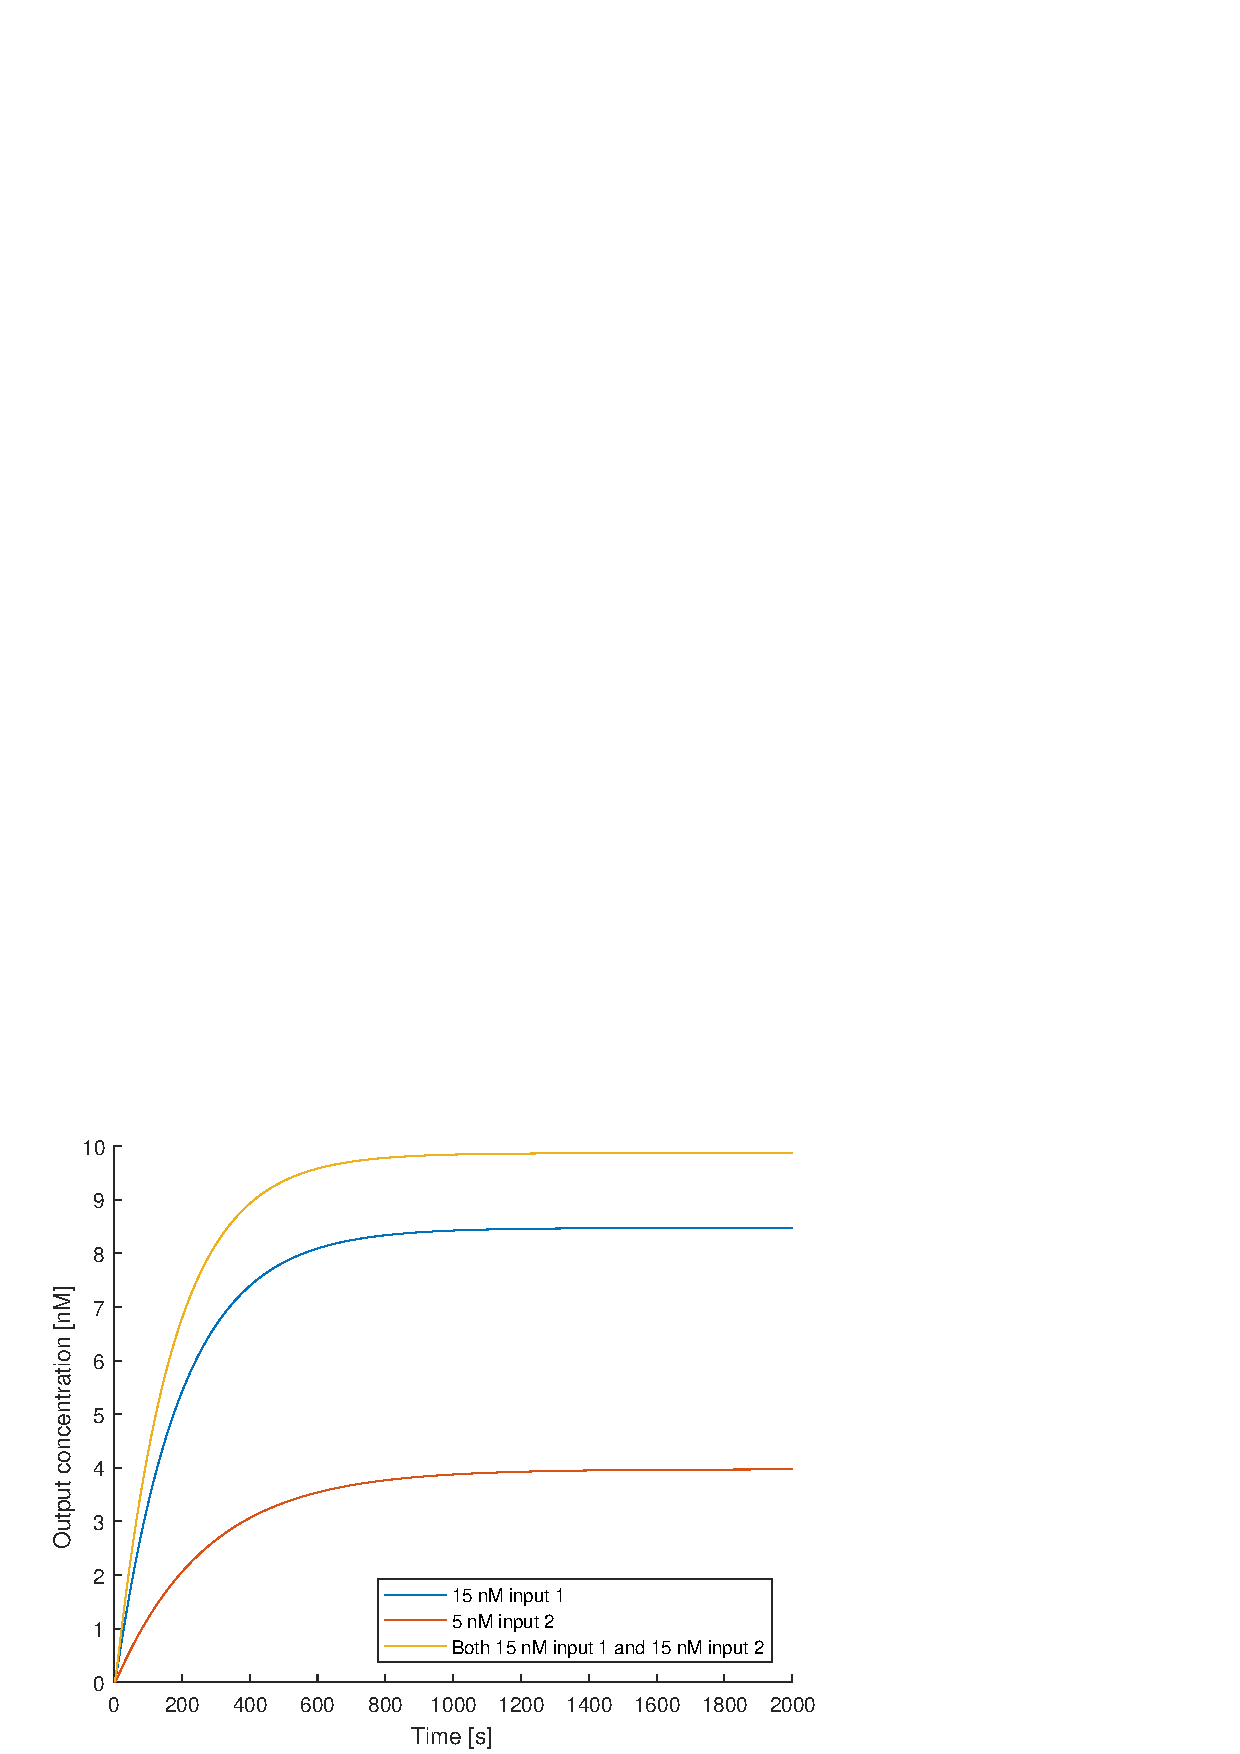
\includegraphics[width=\linewidth]{images/integration.png}
\caption{Time analysis of the concentration of the output strand. The concentration of the integration gate is 20 nM. The first input of 15 nM increases the output strand concentration, compared to the second input of 5 nM. When both strands are added the concentration of output increases further.}
\label{}
\end{subfigure}
\label{seesaw_integration}
\end{figure}

\begin{figure}[H]
\centering
\includegraphics[width=\columnwidth]{images/seesaw_weight.png}
\caption{}
\label{seesaw_weight}
\end{figure}

A problem with this approach to weighting, is that the inputs can only contribute positively to the sum. In silico neural networks can use negative weights to simulate inhibitory synaptic connections, and is needed to implement many kind of boolean functions. The in vitro network can't have negative concentrations of input sequences, so other approaches have to be considered.

WRITE STUFF ABOUT DUAL RAIL LOGIC HERE

\subsubsection{Training}
WRITE STUFF ABOUT TRAINING

  \chapter{Method}
  % !TEX root = ../main.tex
\section{Method}

\subsection{Design}

\begin{table}
\begin{adjustbox}{width=\columnwidth}
\begin{tabular}{llll}
\hline
\textbf{Name}      & \textbf{Short} & \textbf{Sequence}                                           & \textbf{Length} \\
\hline
T7 promoter        & 0          & GGTAATACGACTCACTATAG                                           & 20     \\
Short 1            & 1          & CCTCAAGGAGCTTCAGTCTAGCCCTATAGTGAGTCGTATTACC                    & 43     \\
Short 2            & 2          & CTCCTTGAGGCACATAACTCCCCTATAGTGAGTCGTATTACC                     & 42     \\
Short 3            & 3          & CACATAACTCTACTAAATCTCCCTATAGTGAGTCGTATTACC                     & 42     \\
Short 4            & 4          & GAGTTATGTGCCTCAAGGAGCCCTATAGTGAGTCGTATTACC                    & 42     \\
Short 5            & 5          & AGATTTAGTAGAGTTATGTGCCCTATAGTGAGTCGTATTACC                     & 42     \\
Long 1             & 6          & GTCAATTCGCCTCAAGGAGCTTCAGTCTAGCCCTATAGTGAGTCGTATTACC           & 52     \\
Long 2             & 7          & GCTCCTTGAGGCGAATTGACCCATCTTCATTCTACTCCTACCCTATAGTGAGTCGTATTACC & 62     \\
Long 3             & 8          & CCATCTTCATTCTACTCCTATACCTCAATCCCCTATAGTGAGTCGTATTACC           & 52     \\
Long 4             & 9          & TAGGAGTAGAATGAAGATGGGTCAATTCGCCTCAAGGAGCCCCTATAGTGAGTCGTATTACC & 62     \\
Long 5             & 10         & GATTGAGGTATAGGAGTAGAATGAAGATGGCCCTATAGTGAGTCGTATTACC           & 52     \\
% Beacon fluorophore & 11         & CGGCTAGACTGAA                                                  & 13     \\
% Beacon quencher    & 12         & CCTCAAGGAGCTTCAGTCTAGCCG                                       & 24 \\
\hline
\end{tabular}
\end{adjustbox}
\caption{Sequences and names of the DNA strands used for transcription.}
\label{dna_strands}
\end{table}

\begin{table}
\begin{adjustbox}{width=\columnwidth}
\begin{tabular}{llll}
\hline
\textbf{Name}      & \textbf{Short} & \textbf{Sequence}                                           & \textbf{Length} \\
\hline
Short 1            & 1          & GGCUAGACUGAAGCUCCUUGAGG                    & 23     \\
Short 2            & 2          & GGGAGUUAUGUGCCUCAAGGAG                     & 22     \\
Short 3            & 3          & GGAGAUUUAGUAGAGUUAUGUG                     & 22     \\
Short 4            & 4          & GGCUCCUUGAGGCACAUAACUC                     & 22     \\
Short 5            & 5          & GGCACAUAACUCUACUAAAUCU                     & 22     \\
Long 1             & 6          & GGCUAGACUGAAGCUCCUUGAGGCGAAUUGAC           & 32     \\
Long 2             & 7          & GGUAGGAGUAGAAUGAAGAUGGGUCAAUUCGCCUCAAGGAGC & 42     \\
Long 3             & 8          & GGGAUUGAGGUAUAGGAGUAGAAUGAAGAUGG           & 32     \\
Long 4             & 9          & GGGCUCCUUGAGGCGAAUUGACCCAUCUUCAUUCUACUCCUA & 42     \\
Long 5             & 10         & GGCCAUCUUCAUUCUACUCCUAUACCUCAAUC           & 32     \\
% Beacon fluorophore & 11         & CGGCTAGACTGAA                                                  & 13     \\
% Beacon quencher    & 12         & CCTCAAGGAGCTTCAGTCTAGCCG                                       & 24 \\
\hline
\end{tabular}
\end{adjustbox}
\caption{Sequences and names of the transcribed RNA strands.}
\label{rna_strands}
\end{table}

\subsection{Transcription}

The oligos from IDT was dissolved in TE buffer [PROTOCOL] to an approximate concentration of 120 $\mu$M, based on the quantity of substance written on the tubes. The final concentration desired was 100 $\mu$M, but due to a risk of inaccurate substance quantities, the dissolved concentration was chosen to be slightly above. The oligos could then be further diluted after measuring their absorbance on the Nanodrop.

After dissolving the oligos, the absorbance of each sample was measured on the Nanodrop in triplets. A program was written which can take the .csv output of the Nanodrop, and calculate the concentration based on each strands extinction coefficient \cite{nanodropimport}.

The measured concentrations (figure \ref{oligo_concentrations}) was used to dilute the samples further, to a concentration of 100 $\mu$M.

To anneal the templates to the promoter, each of the template strands was mixed with equal amounts of promoter strand in annealing buffer [PROTOCOL], to a final concentration of 1 $\mu$M. The mixed samples were then heated to 90$^\circ$ C for 5 minutes, and left to cool down to room temperature.

To check if samples annealed properly, they were run on a 20\% native PAGE gel for 3 hours. Each lane was loaded with 50 $\mu$l sample, and 10 $\mu$l native loading buffer [PROTOCOL]. Afterwards the gel was stained in SYBR Gold, and visualised on the Typhoon scanner [PROTOCOL]. The result of the scan can be seen in figure \ref{fig:promoter_annealing_gel}.

\begin{figure}[H]
\centering
\includegraphics[width=\columnwidth]{images/promoter_annealing_gel.png}
\caption{Typhoon scan of SYBR Gold stained native PAGE gel, with the annealed templates and promoter strands. The lanes are labelled by which strands are annealed (see table \ref{dna_strands}).}
\label{fig:promoter_annealing_gel}
\end{figure}

As can be seen in figure \ref{fig:promoter_annealing_gel}, the darkest bands is the annealed samples. The samples for the short translator runs as about the same size, while there is bigger variation in the long translator samples, as expected based on table \ref{dna_strands}. The exact positions of the long translator samples does not match with the sequence length, though this can be explained by secondary structures of the single-stranded part of the sample. The shorter bands visible below, is probably excess promoter, other secondary structures, and shorter sequences from synthesis errors. No lane with ladder was run, so the exact position of the bands can't be commented on.

To get the desired RNA sequences, a transcription reaction was run with each of the annealed DNA templates, according to table \ref{transcription1}.

\begin{table}\centering
\begin{tabular}{llll}
  \hline
                       & \textbf{Initial conc.} & \textbf{Final conc.} & \textbf{Volume} \\ \hline
  Transcription buffer & 10X                    & 1X                   & 10 \si{\micro}L           \\
  DTT                  & 100 mM                 & 10 mM                & 10 \si{\micro}L           \\
  NTP mix              & 25 mM                  & 2.5 mM               & 10 \si{\micro}L           \\
  Template             & 500 nM                 & 50 nM                & 10 \si{\micro}L           \\
  T7 RNA polymerase    &                        &                      & 1 \si{\micro}L            \\
  Nuclease-free water  &                        &                      & 59 \si{\micro}L           \\
  Total                &                        &                      & 100 \si{\micro}L          \\ \hline
\end{tabular}
\caption{Mixing of compounds for the first transcription done on the templates for both the short and long translater.}
\label{transcription1}
\end{table}

The samples were left overnight at 37$^\circ$ C. The day after, 1 \si{\micro}L of RNAse free DNAse was added to the samples, and heated for 37$^\circ$ C for an hour. Afterwards, 100 ul of denaturing loading buffer was added to each sample, and 10 ul of the DNA 0 and DNA 5 strands was mixed with 10 ul of denaturing loading buffer, and heated for 5 minutes at 90$^\circ$ C.

To purify the RNA, the transcribed sequences and controls were run on a 20\% denaturing PAGE gel, for 4 hours at 20 W.

The RNA product should be visible in UV shadowing, but no product was visible. The gel was then stained with SYBR Gold and scanned on the Typhoon [PROTOCOL]. The result can be seen in figure \ref{transcription_1}.

\begin{figure}[H]
\centering
\includegraphics[width=200]{images/translator_transcription_1.png}
\caption{Typhoon scan of SYBR Gold stained native PAGE gel, with the transcribed RNA strands in lanes 1-10, and controls in 11 and 12. The lanes are labelled by which strands are annealed (see \tref{rna_strands}). The asterix refers to the DNA strands in \tref{dna_strands}.}
\label{transcription_1}
\end{figure}

As can be seen in \fref{transcription_1}, the gel wasn't stained long enough, so after restaining it in SYBR Gold, it was scanned again.

\begin{figure}[H]
\centering
\includegraphics[width=200]{images/translator_transcription_2.png}
\caption{Typhoon scan of SYBR Gold stained native PAGE gel, with the transcribed RNA strands in lanes 1-10, and controls in 11 and 12. The lanes are labelled by which strands are annealed (see table \ref{rna_strands}). The asterix refers to the DNA strands in table \ref{dna_strands}.}
\label{transcription_2}
\end{figure}

The lanes 1-10 in \fref{transcription_2} does not show distinct bands. There seems to be more product from the long translator transcriptions (lanes 6-10), than in the short ones (lanes 1-5). Even the controls which were loaded in equal amounts does not show up in equal strength. Since the gel from the DNA annealing was run without any controls, it was difficult to see if there was any errors in the annealing. Another 20\% native PAGE gel was run with the annealed DNA, using the single stranded oligos as control. To simplify the experiment while trying to the find the error, only the short translator sequences were used.

\begin{figure}[H]
\centering
\includegraphics[width=200]{images/translator_annealing_2.png}
\caption{The annealed oligos together with controls and a 10 nt ladder. The lanes are labelled with the oligo names given in \tref{dna_strands}. The plus symbol denotes which strands are annealed.}
\label{translator_annealing_2}
\end{figure}

The results of \fref{translator_annealing_2} still shows that the templates have annealed with the promoter, and runs as about 40-50 bp. The expected size is around 60 bp (sum of promoter and template), but it is difficult to say how a partly annealed structure will run on a native gel. The new gel does however show that the bands in the annealed lanes below the assumed product, might not be excess promoter. The promoter is seen in the second lane, and lies below the bands in the annealed structure thought to be excess promoter. The bands below the product might be due to secondary structures of each of the template strands, but comparing with \fref{short_secondary_structures}, the band in the 5+0 lane would be expected to be less visible, as strand 5 has no secondary structure.

Despite the unexplained bands from the annealing, a new transcription was run on the short template strands to see if better results could be attained.

  \chapter{Results and discussion}
  % !TEX root = ../main.tex

\section{Results}
To test the perceptron compiling and training, 5 different truth tables were used, ranging from 2 to 3 inputs. The correct output was reached after 16-23 iterations of the learning algorithm. Input sizes greater than 3 was not tested, as the training time increases exponentially in time with the input size.


\begin{figure}[H]
  \begin{subfigure}[t]{.49\columnwidth}
    \begin{tabular}[b]{ccc}
      \hline
    \multicolumn{1}{l}{\textbf{Input 1}} & \multicolumn{1}{l}{\textbf{Input 2}} & \multicolumn{1}{l}{\textbf{Output}} \\
    \hline
    0                                    & 0                                    & 0                                   \\
    0                                    & 1                                    & 0                                   \\
    1                                    & 0                                    & 0                                   \\
    1                                    & 1                                    & 1 \\
    \hline
    \end{tabular}
    \caption{Truth table for the 2-input AND gate.}
    \label{and_table}
\end{subfigure}
\hfill
\begin{subfigure}[t]{.49\columnwidth}
  \centering
\includegraphics[width=\linewidth]{images/and_simulation.png}
\caption{.}
\label{}
\end{subfigure}
\caption{Simulation results of the trained 2-input AND gate. The network is trained to activate when both of the inputs are active. The correct output was obtained after 21 iterations of the training algorithm, with a weight of 1.9 for all inputs, and a threshold of 10.}
\end{figure}

\begin{figure}[H]
  \begin{subfigure}[t]{.49\columnwidth}
    \begin{tabular}[b]{ccc}
      \hline
    \multicolumn{1}{l}{\textbf{Input 1}} & \multicolumn{1}{l}{\textbf{Input 2}} & \multicolumn{1}{l}{\textbf{Output}} \\
    \hline
    0                                    & 0                                    & 0                                   \\
    0                                    & 1                                    & 1                                   \\
    1                                    & 0                                    & 1                                   \\
    1                                    & 1                                    & 1 \\
    \hline
    \end{tabular}
    \caption{Truth table for the 2-input OR gate.}
    \label{and_table}
\end{subfigure}
\hfill
\begin{subfigure}[t]{.49\columnwidth}
  \centering
\includegraphics[width=\linewidth]{images/or_simulation.png}
\caption{.}
\label{}
\end{subfigure}
\caption{Simulation results of the trained 2-input OR gate. The network is trained to activate when one of the inputs is active. The correct output was obtained after 22 iterations of the training algorithm, with a weight of 2.1 for all inputs, and a threshold of 10.}
\end{figure}

\begin{figure}[H]
  \begin{subfigure}[t]{.49\columnwidth}
    \begin{tabular}[b]{cccc}
      \hline
    \multicolumn{1}{l}{\textbf{Input 1}} & \multicolumn{1}{l}{\textbf{Input 2}} & \multicolumn{1}{l}{\textbf{Input 3}} & \multicolumn{1}{l}{\textbf{Output}} \\
    \hline
    0 & 0                                    & 0                                    & 0                                   \\
    0 & 0                                    & 1                                    & 0                                   \\
    0 & 1                                    & 0                                    & 0                                   \\
    0 & 1                                    & 1                                    & 0                                   \\
    1 & 0                                    & 0                                    & 0                                   \\
    1 & 0                                    & 1                                    & 0                                   \\
    1 & 1                                    & 0                                    & 0                                   \\
    1 & 1                                    & 1                                    & 1                                   \\

    \hline
    \end{tabular}
    \caption{Truth table for the 3-input AND gate.}
    \label{and_table}
\end{subfigure}
\hfill
\begin{subfigure}[t]{.49\columnwidth}
  \centering
\includegraphics[width=\linewidth]{images/and_simulation_3input.png}
\caption{.}
\label{}
\end{subfigure}
\caption{Simulation results of the trained 3-input AND gate. The network is trained to activate when all of the inputs are active. The correct output was obtained after 14 iterations of the training algorithm, with a weight of 1.2 for all inputs, and a threshold of 10.}
\end{figure}

\begin{figure}[H]
  \begin{subfigure}[t]{.49\columnwidth}
    \begin{tabular}[b]{cccc}
      \hline
    \multicolumn{1}{l}{\textbf{Input 1}} & \multicolumn{1}{l}{\textbf{Input 2}} & \multicolumn{1}{l}{\textbf{Input 3}} & \multicolumn{1}{l}{\textbf{Output}} \\
    \hline
    0 & 0                                    & 0                                    & 0                                   \\
    0 & 0                                    & 1                                    & 1                                   \\
    0 & 1                                    & 0                                    & 1                                   \\
    0 & 1                                    & 1                                    & 1                                   \\
    1 & 0                                    & 0                                    & 1                                   \\
    1 & 0                                    & 1                                    & 1                                   \\
    1 & 1                                    & 0                                    & 1                                   \\
    1 & 1                                    & 1                                    & 1                                   \\

    \hline
    \end{tabular}
    \caption{Truth table for the 3-input 1-OR gate.}
    \label{and_table}
\end{subfigure}
\hfill
\begin{subfigure}[t]{.49\columnwidth}
  \centering
\includegraphics[width=\linewidth]{images/or_1_simulation_3input.png}
\caption{.}
\label{}
\end{subfigure}
\caption{Simulation results of the trained 3-input 1-OR gate. The network is trained to activate when at least 1 of the inputs is active. The correct output was obtained after 16 iterations of the training algorithm, with a weight of 1.3 for all inputs, and a threshold of 10.}
\end{figure}

\begin{figure}[H]
  \begin{subfigure}[t]{.49\columnwidth}
    \begin{tabular}[b]{cccc}
      \hline
    \multicolumn{1}{l}{\textbf{Input 1}} & \multicolumn{1}{l}{\textbf{Input 2}} & \multicolumn{1}{l}{\textbf{Input 3}} & \multicolumn{1}{l}{\textbf{Output}} \\
    \hline
    0 & 0                                    & 0                                    & 0                                   \\
    0 & 0                                    & 1                                    & 0                                   \\
    0 & 1                                    & 0                                    & 0                                   \\
    0 & 1                                    & 1                                    & 1                                   \\
    1 & 0                                    & 0                                    & 0                                   \\
    1 & 0                                    & 1                                    & 1                                   \\
    1 & 1                                    & 0                                    & 1                                   \\
    1 & 1                                    & 1                                    & 1                                   \\

    \hline
    \end{tabular}
    \caption{Truth table for the 3-input 2-OR gate.}
    \label{and_table}
\end{subfigure}
\hfill
\begin{subfigure}[t]{.49\columnwidth}
  \centering
\includegraphics[width=\linewidth]{images/or_2_simulation_3input.png}
\caption{.}
\label{}
\end{subfigure}
\caption{Simulation results of the trained 3-input 2-OR gate. The network is trained to activate when at least 2 of the inputs is active. The correct output was obtained after 15 iterations of the training algorithm, with a weight of 1.3 for all inputs, and a threshold of 10.}
\end{figure}



  \chapter{Conclusion}
  % !TEX root = ../main.tex

Since it was not possible to transcribe the RNA needed for testing the RNA translator, it is not possible to conclude anything from the results. The experiment was almost identical to the original article, and there is nothing to suggest that the strand displacement shouldn't have worked using RNA instead of DNA \cite{Picuri2009}. The original article even uses RNA as the input for the DNA translators.

The simulations of the neural network did show some promising results. It was possible to create multiple perceptrons of varying input size, and train them to different truth tables (\cref{2_and,2_or,3_and,3_1_or,3_2_or}). The system requires no input from the user after having defined the desired truth table.

The perceptron in this experiment is still only a stripped down version of the networks in the original article \cite{Qian2011}, as it was not possible to apply the dual-rail logic needed for avoiding negative weights. It was not possible to translate the input sequences using Nupack either. Furthermore, the perceptrons trained in this experiment, could have been made much simpler by the logic gate system the authors of the original article designed recently \cite{Thubagere2017}. The only novel thing that came out of this experiment was the simplified training algorithm for the perceptrons without dual-rail logic.

There is also the problem of applying the simulations to in vitro reactions. The original paper found some general guidelines for adjusting the concentrations that seemed to work for some networks, but it can't be expected that the sequences and concentrations found in the simulation will always work in vitro. In the original paper, they also express concern for moving to in vivo.

Still, the preliminary work done in this experiment could in theory be used to create a generic method for designing RNA/DNA detection kits. With some more work, the training algorithm and input translation could be combined, and tested in vitro.


  \bibliographystyle{unsrt}
  \bibliography{references}

  \appendix
  \chapter{Appendix}
  % !TEX root = ../main.tex
\section{Appendix}

\begin{figure}[H]
\centering
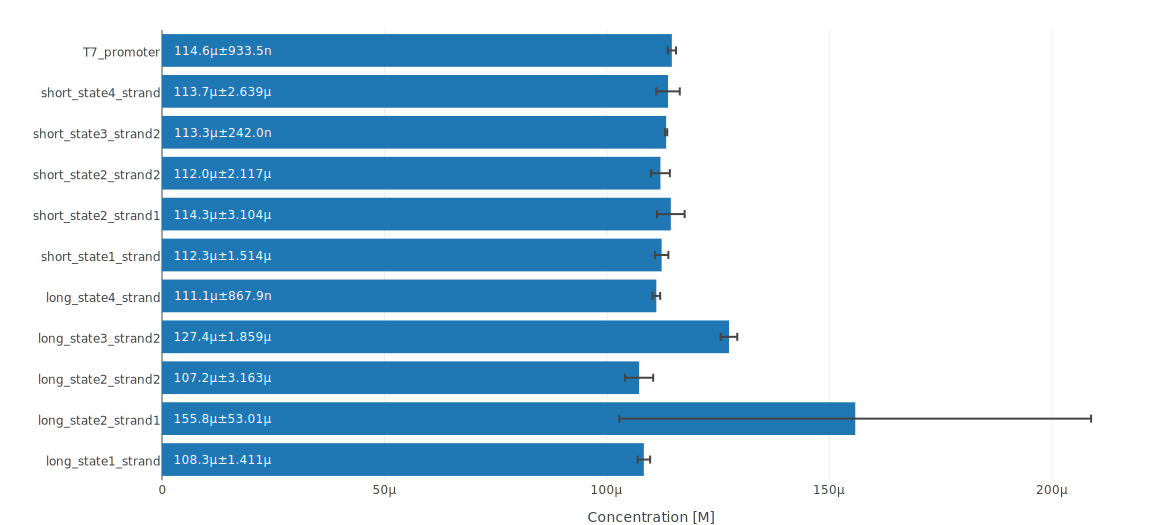
\includegraphics[width=\columnwidth]{images/oligo_concentrations.png}
\caption{}
\label{oligo_concentrations}
\end{figure}


\end{document}
